\documentclass[a4paper,10pt]{article}

%%%%%%%%%%%%%%%%%%%%%%%%%%%%%%%%%%%%%%%%%%%%%%%%%%
% Los paquetes permiten ampliar las capacidades de LaTeX.                     %
%%%%%%%%%%%%%%%%%%%%%%%%%%%%%%%%%%%%%%%%%%%%%%%%%%
% Paquete para inclusión de gráficos.
\usepackage{graphicx}

% Paquete para definir la codificación del conjunto de caracteres usado
\usepackage[utf8]{inputenc}

% Paquete para definir el idioma usado.
\usepackage[spanish]{babel}

% Paquete para introducir codigo de programacion
\usepackage{listings}

 % Para poder introducir otrod PDFs
\usepackage{pdfpages}

% Para inseratar imagenes
\usepackage{graphicx}
\usepackage{subfigure}

\usepackage{mips}



% Título principal del documento.
\title{\textbf{Trabajo práctico 1: conjunto de instrucciones MIPS}}


% Información sobre los autores.
\author{Augusto Arturi (\#97498)\\
\texttt{turitoh@gmail.com}\\
\\
Matias Rozanec (\#97404)\\            \texttt{rozanecm@gmail.com}\\
\\
Agustin Miguel Payaslian (\#96885)\\            \texttt{payas17@hotmail.com}\\
\\
\normalsize{Grupo Nro. \# - 2do. Cuatrimestre de 2017}\\
\\
\\
\normalsize{66.20 Organización de Computadoras}\\
\normalsize{Facultad de Ingeniería, Universidad de Buenos Aires}\\
}
\date{5/10/2017}

\lstset{
  language=bash,
  basicstyle=\ttfamily
}
\lstdefinestyle{numbers} {numbers=left, stepnumber=1, numberstyle=\tiny, numbersep=10pt}

\lstdefinestyle{MyFrame}{backgroundcolor=\color{white},frame=shadowbox}

\lstdefinestyle{noframe} {language=bash,style=MyFrame,frame=none}

\lstdefinestyle{customc}{
  belowcaptionskip=1\baselineskip,
  breaklines=true,  
  xleftmargin=-5em,
  language=C,
  showstringspaces=false,
  basicstyle=\footnotesize\ttfamily,
  keywordstyle=\bfseries\color{green!40!black},
  commentstyle=\itshape\color{purple!40!black},
  identifierstyle=\color{blue},
  stringstyle=\color{orange},
  numberstyle=\tiny,
  resetmargins=true,
  style=MyFrame,
  numbers=left,                   % where to put the line-numbers
  numberstyle=\tiny\color{gray},
}

\lstdefinestyle{customasm}{
  belowcaptionskip=1\baselineskip,
  frame=L,
  xleftmargin=-5em,
  language=[x86masm]Assembler,
  basicstyle=\footnotesize\ttfamily,
  commentstyle=\itshape\color{purple!40!black},
  style=MyFrame,
}

\definecolor{dkgreen}{rgb}{0,0.6,0}
\definecolor{gray}{rgb}{0.5,0.5,0.5}
\definecolor{mauve}{rgb}{0.58,0,0.82}

\lstdefinestyle{mips}{ %
  language=[mips]Assembler,       % the language of the code
  basicstyle=\footnotesize,       % the size of the fonts that are used for the code
  numbers=left,                   % where to put the line-numbers
  numberstyle=\tiny\color{gray},  % the style that is used for the line-numbers
  stepnumber=1,                   % the step between two line-numbers. If it's 1, each line 
                                  % will be numbered
  numbersep=5pt,                  % how far the line-numbers are from the code
  backgroundcolor=\color{white},  % choose the background color. You must add \usepackage{color}
  showspaces=false,               % show spaces adding particular underscores
  showstringspaces=false,         % underline spaces within strings
  showtabs=false,                 % show tabs within strings adding particular underscores
  frame=single,                   % adds a frame around the code
  rulecolor=\color{black},        % if not set, the frame-color may be changed on line-breaks within not-black text (e.g. commens (green here))
  tabsize=4,                      % sets default tabsize to 2 spaces
  captionpos=b,                   % sets the caption-position to bottom
  breaklines=true,                % sets automatic line breaking
  breakatwhitespace=false,        % sets if automatic breaks should only happen at whitespace
  title=\lstname,                 % show the filename of files included with \lstinputlisting;
    xleftmargin=-5em,                                % also try caption instead of title
  keywordstyle=\color{blue},          % keyword style
  commentstyle=\color{dkgreen},       % comment style
  stringstyle=\color{mauve},         % string literal style
  escapeinside={\%*}{*)},            % if you want to add a comment within your code
  morekeywords={*,...}   
            % if you want to add more keywords to the set
}


\begin{document}


% Inserta el título.
\maketitle
% Quita el número en la primer página.

% Resumen

\begin{figure}[!htp]
\centering
\includegraphics[scale=1]{../../../Imagenes/fiubalogo2.png} 

\end{figure}
\thispagestyle{empty}
\newpage

\begin{abstract}
El objetivo del siguiente trabajo es familiarizarse con el conjunto de instrucciones MIPS32 y el concepto de ABI, escribiendo un programa portable que resuelva los problemas de minimo común múltiplo (mcm) y el máximo común divisor (mcd) entre dos números.
\end{abstract}


\section{Introducción}
Aquí se comenta en forma escueta cómo está constituido el presente informe, donde  básicamente  se  encuentran  dos  secciones  principales: Desarrollo y Conclusiones.\\
En Desarrollo se encuentran breves comentarios sobre la implementacion del algoritmo como tambien, las corridas de prueba del programa. En la seccion conclusiones se discuten los resultados obtenidos.

\section{Desarrollo}

\subsection{Implementación}
A la hora de desarrollar el programa se utilizó el criterio establecido por la consigna del práctico: por un lado realizar una API donde gran parte del programa es implementado en lenguaje C, mientras que las funciones \textit{mcd(m, n)} y \textit{mcm(m, n)} son implementadas también en assembly con el fin de proveer soporte especifico en nuestra plataforma principal de desarrollo, NetBSD/pmax. A la hora de brindar portabilidad entre sistemas operativos, también se debe realizar otra versión la cual esté desarrollada en su totalidad en C.


\subsection{API}

El algoritmo utilizado es el de Euclides. La estrategia de la cual se partió para realizar la implentación en assembly fue realizar todas las validaciones correspondientes a m y n fuera de las funciones \textit{mcd(m, n)} y \textit{mcm(m, n)}, utilizando estas dos únicamente para
efectuar las operaciones específicas de cada algoritmo necesarias con el fin de obtener los resultados deseados.Cabe destacar que primero se realizó la version portable, es decir aquella que fue desarrollada en C en su totalidad, luego se procedió haciendo la traducción de la misma en asm.

	La función mcd(m,n) fue realizada de manera recursiva.
	
	Durante el desarrollo de la misma se respeta la ABI, los argumentos almacenados por el callee son almacenados en el argument area del stack.
	
\subsection{Compilacion}


\begin{lstlisting}[style=noframe]
root@:~# gcc -Wall -std=c99 -lm main.c my_assembly.S -o common
\end{lstlisting}
\newpage
\subsection{Corridas de prueba}

A continuacion se demuestran las corridas de prueba con todos los casos posibles.
\begin{lstlisting}[style=MyFrame]
root@:~# ./common -h
Usage:
        common -h 
        common -v 
        common [options] M N 
Options:
        -h, --help      Print usage information.
        -V, --version   Prints version information.
        -o, --output    Path to output file.
        -d  --divisor   Just the divisor
        -m  --multiple  Just the multiple
Examples:
        common -o - 256 192
        
root@:~# ./common --version
API Version 1.0
root@:~# ./common -m -o 256 192
768
root@:~# ./common -d -o 256 192
64
root@:~# ./common -o EJEMPLO 256 192

\end{lstlisting}
En esta última corrida se guardan en un archivo (EJEMPLO) los resultados de mcm y mcd.


A continuación, los ejemplos pedidos
\begin{lstlisting}[style=MyFrame]
root@:~# ./common 5 10
10
5
root@:~# ./common 256 192
768
64
root@:~# ./common 1111 1294
1437634
1
\end{lstlisting}

Aqui ejemplos con datos de entrada incorrectos, los primeros dos por rango invalido y el ultimo por ingresar un valor negativo.
\begin{lstlisting}[style=MyFrame]
root@:~# ./common 111111111111 123456
strtol: Result too large or too small
root@:~# ./common 0 10
root@:~# ./common -2 10              
common: unknown option -- 2

\end{lstlisting}

\subsection{Diagrama de stack}

Se muestra el stack creado, el mismo es identico para las funciones mcm o mcd, ya que las dos son \textbf{no hoja} 

\begin{figure}[!htp]
\centering
\includegraphics[scale=0.4]{../../../Imagenes/stack_generico.png} 
\end{figure}

A continuacion un caso en el cual se hace un seguimiento del stack para el siguiente comando:

\textbf{./common 256 198} 

\begin{figure}[!htp]
\centering
\includegraphics[scale=0.5]{../../../Escritorio/mcd_mcm.png} 
\end{figure}
\newpage

\section{Conclusiones}

En este trabajo práctico se incorporaron nuevos conceptos de importante valor tanto para el curso de la materia como para la carrera en sí. Por un lado se llevó a la práctica la programación con el conjunto de instrucciones de MIPS32, lo cual a la hora de hacerlo en una computadora conlleva una dificultad extra consistente en  el ensamblado y compilación, verificación de todas las advertencias obtenidas y la corrección de las mismas, ya que algunas de éstas permitieron lograr los resultados esperados a la hora de correr el ejecutable. Además, la implentación se realizó teniendo en cuenta la ABI propuesta, la cual se tuvo presente en todo momento a lo largo del desarrollo del práctico.

Un factor que se considera de gran valor fue el de realizar el diagrama de stack. Al ser la función recursiva, se observa cómo el stack aumenta su tamaño con gran facilidad, dejando explícito lo explicado en clase con otros ejemplos, como el caso del cálculo del factorial de un número de forma recursiva. Se considera que el seguimiento del stack para el ejemplo dado ayuda a la comprensión tanto de la ABI como del manejo de memoria.

Finalmente se considera que una vez realizado este trabajo se logra comprender cómo funciona realmente una computadora a bajo nivel y qué dificultades implica a la hora de implementar una solucion en lenguaje ensamblador. Se analizó el código generado por gcc sin optimizaciones (-O0) y se observa que el manejo de memoria es distinto al realizado, generando éste instrucciones innecesarias
de load y store, que al evitarlas por nuestra propia cuenta estamos optimizando el código. También se intentó ver una comparación de tiempos de ejecución entre la versión portable vs API, sin embargo los resultados no fueron apreciables ya que ambas se ejecutaron tan rápido que el clock no observa diferencia entre estas.

\section{Apendice A, codigo fuente}


\subsection{Version 1, portable}
\textbf{main.c}
\begin{lstlisting}[style=customc]
#include <stdlib.h>
#include <stdio.h>
#include <getopt.h>
#include <limits.h>
#include <errno.h>

/* define max input. Number is max supported for 32 bit unsigned int */
#define MAX_INPUT UINT_MAX

void print_help_data(){
    printf("Usage:\n "
                   "\tcommon -h \n"
                   "\tcommon -v \n"
                   "\tcommon [options] M N \n"
                   "Options:\n"
                   "\t-h, --help \tPrint usage information.\n"
                   "\t-V, --version \tPrints version information.\n"
                   "\t-o, --output\tPath to output file.\n"
                   "\t-d  --divisor\tJust the divisor\n"
                   "\t-m  --multiple\tJust the multiple\n"
                   "Examples:\n"
                   "\tcommon -o - 256 192\n");
}

void print_version_info(){
    printf("Version 1.0\n");
}

int mcd(int a, int b) {
    /* Precondition: a > b */

    if (b == 0){
        return a;
    } else {
        return mcd(b, a % b);
    }
}

int mcm(const int a, const int b){
    return abs(a * b) / mcd(a, b);
}

short int check_range(unsigned long int a, unsigned long int b){
    /* This function tests the input numbers to be in range [2, MAX_INPUT].
     * Return values:
     *      0: Success.
     *      1: Failure.
     * */
    if ((a >= 2) && (a <= MAX_INPUT) && (b >= 2) && (b <= MAX_INPUT)){
        /* Success */
        return 0;
    }

    /* failure */
    return 1;
}

void process_input_numbers(unsigned long int *a, unsigned long int *b,
                           char *input1, char *input2){
    /* Process input numbers */
    errno = 0;
    char* endptr = NULL;
    *a = strtoul(input1, &endptr, 10);
    /* error checking performed according to strtol man page */
    if ((errno == ERANGE && (*a == LONG_MAX || *a == LONG_MIN))
        || (errno != 0 && *a == 0)) {
        perror("strtol");
        exit(EXIT_FAILURE);
    }

    *b = strtoul(input2, &endptr, 10);
    /* error checking performed according to strtol man page */
    if ((errno == ERANGE && (*b == LONG_MAX || *b == LONG_MIN))
        || (errno != 0 && *b == 0)) {
        perror("strtol");
        exit(EXIT_FAILURE);
    }

    /* make sure a > b
     * although this is not strictly necessary, we make it this way so it is
     * easier to follow */
    if (a < b){
        unsigned long int aux = *a;
        *a = *b;
        *b = aux;
    }

    if (check_range(*a, *b) == 1){
        exit(EXIT_FAILURE);
    }
}

void print_mcm(unsigned int a, unsigned int b, char* path){
    /* According to ASCII table, 45 is the '-' char.
     * Source: http://www.asciitable.com/ */
    if (*path == 45){
        /* output to stdout */
        printf("%i\n", mcm(a, b));
    }else{
        FILE* file = fopen(path, "a");
        /* error checking */
        if (file == NULL){
            exit(EXIT_FAILURE);
        }

        fprintf(file, "%i\n", mcm(a, b));

        fclose(file);
    }
}

void print_mcd(unsigned int a, unsigned int b, char* path){
    /* According to ASCII table, 45 is the '-' char.
     * Source: http://www.asciitable.com/ */
    if (*path == 45){
        /* output to stdout */
        printf("%i\n", mcd(a, b));
    }else{
        FILE* file = fopen(path, "a");
        /* error checking */
        if (file == NULL){
            exit(EXIT_FAILURE);
        }

        fprintf(file, "%i\n", mcd(a, b));

        fclose(file);
    }
}

int main(int argc, char* argv[]){
    unsigned long int a, b;
    static struct option long_options[] = {
            {"help", 	    no_argument, 		0, 'h' },
            {"version",	    no_argument, 		0, 'v' },
            {"output",	    required_argument,	0, 'o' },
            {"divisor",	    no_argument,	    0, 'd' },
            {"multiple",	no_argument,    	0, 'm' },
            {0,			    0,					0,  0  }
    };
    int option_index = 0;
    int c = getopt_long(argc, argv, "hvo:dm", long_options, &option_index);
    switch (c){
        case 'h':
            print_help_data();
            break;
        case 'v':
            print_version_info();
            break;
        case 'o':
            process_input_numbers(&a, &b, argv[argc-2], argv[argc-1]);
            print_mcm(a, b, optarg);
            print_mcd(a, b, optarg);
            break;
        case 'd':
            process_input_numbers(&a, &b, argv[argc-2], argv[argc-1]);
            print_mcd(a, b, "-");
            break;
        case 'm':
            process_input_numbers(&a, &b, argv[argc-2], argv[argc-1]);
            print_mcm(a, b, "-");
            break;
        default:
            process_input_numbers(&a, &b, argv[argc-2], argv[argc-1]);
            print_mcm(a, b, "-");
            print_mcd(a, b, "-");
    }

    exit(EXIT_SUCCESS);
}
\end{lstlisting}

\subsection{Version 2, API}

\textbf{main.c}
\begin{lstlisting}[style=customc]
#include <stdlib.h>
#include <stdio.h>
#include <getopt.h>
#include <errno.h>
#include "my_assembly.h"

/* define max input. Number is max supported for 32 bit unsigned int */
#define MAX_INPUT 2147483647
#define LONG_MAX 4294967295

void print_help_data(){
    printf("Usage:\n "
                   "\tcommon -h \n"
                   "\tcommon -v \n"
                   "\tcommon [options] M N \n"
                   "Options:\n"
                   "\t-h, --help \tPrint usage information.\n"
                   "\t-V, --version \tPrints version information.\n"
                   "\t-o, --output\tPath to output file.\n"
                   "\t-d  --divisor\tJust the divisor\n"
                   "\t-m  --multiple\tJust the multiple\n"
                   "Examples:\n"
                   "\tcommon -o - 256 192\n");
}

void print_version_info(){
    printf("API Version 1.0\n");
}


short int check_range(unsigned long int a, unsigned long int b){
    /* This function tests the input numbers to be in range [2, MAX_INPUT].
     * Return values:
     *      0: Success.
     *      1: Failure.
     * */
    if ((a >= 2) && (a <= MAX_INPUT) && (b >= 2) && (b <= MAX_INPUT)){
        /* Success */
        return 0;
    }

    /* failure */
    return 1;
}

void process_input_numbers(unsigned long int *a, unsigned long int *b,
                           char *input1, char *input2){
    /* Process input numbers */
    errno = 0;
    char* endptr = NULL;
    *a = strtoul(input1, &endptr, 10);
    /* error checking performed according to strtol man page */
    if ((errno == ERANGE && (*a == LONG_MAX))
        || (errno != 0 && *a == 0)) {
        perror("strtol");
        exit(EXIT_FAILURE);
    }

    *b = strtoul(input2, &endptr, 10);
    /* error checking performed according to strtol man page */
    if ((errno == ERANGE && (*b == LONG_MAX ))
        || (errno != 0 && *b == 0)) {
        perror("strtol");
        exit(EXIT_FAILURE);
    }

    /* make sure a > b
     * although this is not strictly necessary, we make it this way so it is
     * easier to follow */
    if (a < b){
        unsigned long int aux = *a;
        *a = *b;
        *b = aux;
    }

    if (check_range(*a, *b) == 1){
        exit(EXIT_FAILURE);
    }
}

void print_mcm(unsigned int a, unsigned int b, char* path){
    /* According to ASCII table, 45 is the '-' char.
     * Source: http://www.asciitable.com/ */
    if (*path == 45){
        /* output to stdout */
        printf("%i\n", mcm(a, b));
    }else{
        FILE* file = fopen(path, "a");
        /* error checking */
        if (file == NULL){
            exit(EXIT_FAILURE);
        }

        fprintf(file, "%i\n", mcm(a, b));

        fclose(file);
    }
}

void print_mcd(unsigned int a, unsigned int b, char* path){
    /* According to ASCII table, 45 is the '-' char.
     * Source: http://www.asciitable.com/ */
    if (*path == 45){
        /* output to stdout */
        printf("%i\n", mcd(a, b));
    }else{
        FILE* file = fopen(path, "a");
        /* error checking */
        if (file == NULL){
            exit(EXIT_FAILURE);
        }

        fprintf(file, "%i\n", mcd(a, b));

        fclose(file);
    }
}

int main(int argc, char* argv[]){
    unsigned long int a, b;
    static struct option long_options[] = {
            {"help", 	    no_argument, 		0, 'h' },
            {"version",	    no_argument, 		0, 'v' },
            {"output",	    required_argument,	0, 'o' },
            {"divisor",	    no_argument,	    0, 'd' },
            {"multiple",	no_argument,    	0, 'm' },
            {0,			    0,					0,  0  }
    };
    int option_index = 0;
    int c = getopt_long(argc, argv, "hvo:dm", long_options, &option_index);
    switch (c){
        case 'h':
            print_help_data();
            break;
        case 'v':
            print_version_info();
            break;
        case 'o':
            process_input_numbers(&a, &b, argv[argc-2], argv[argc-1]);
            print_mcm(a, b, optarg);
            print_mcd(a, b, optarg);
            break;
        case 'd':
            process_input_numbers(&a, &b, argv[argc-2], argv[argc-1]);
            print_mcd(a, b, "-");
            break;
        case 'm':
            process_input_numbers(&a, &b, argv[argc-2], argv[argc-1]);
            print_mcm(a, b, "-");
            break;
        default:
            process_input_numbers(&a, &b, argv[argc-2], argv[argc-1]);
            print_mcm(a, b, "-");
            print_mcd(a, b, "-");
    }

    exit(EXIT_SUCCESS);
}
\end{lstlisting}
\textbf{my\_assembly.h}
\begin{lstlisting}[style=customc]
int mcd(int a, int b);

int mcm(const int a, const int b);
\end{lstlisting}

\textbf{my\_assembly.S}
\begin{lstlisting}[style=mips]
#include <mips/regdef.h>

.globl mcd
.globl mcm


.text
.abicalls
.align 2
.ent mcm


mcm:

    #define mcm_frame_size 32
    #define mcm_frame_ra 24
    #define mcm_frame_fp 20
    #define mcm_frame_gp 16
    #define mcm_frame_2arg 36
    #define mcm_frame_1arg 32
    
    .frame $fp, mcm_frame_size, ra
    /*CREATE STACK FRAME*/
    subu sp, sp, mcm_frame_size
    .cprestore 16
    sw gp, mcm_frame_gp(sp)
    sw $fp, mcm_frame_fp(sp)
    sw ra, mcm_frame_ra(sp)
    move  $fp, sp /* frame pointer at the bottom */
      
    sw a0, mcm_frame_1arg($fp) /*save first argument (int a)*/
    sw a1, mcm_frame_2arg($fp) /*save second argument (int b)*/

    lw t3, mcm_frame_1arg($fp) /* use temporary for a0 value */
    lw t4, mcm_frame_2arg($fp) /* use temporary for a1 value */
   
    mul t3, t3, t4 /* (a * b) */
    
    la t5, mcd /* load address of mcd function */
    jalr t5     /* jump and link to mcd */
    
    div t3, t3, v0 /* (a * b) / mcd(a, b); */

    move v0, t3 /* set result */


    /* PREPARE TO DELETE STACK */
    lw gp, mcm_frame_gp(sp)
    lw $fp, mcm_frame_fp(sp)
    lw ra, mcm_frame_ra(sp)
    addu sp, sp, mcm_frame_size
    jr ra
    
.end mcm
   
.text
.abicalls
.align 2
.ent mcd

mcd:

    #define mcd_frame_size 32
    #define mcd_frame_ra 24
    #define mcd_frame_fp 20
    #define mcd_frame_gp 16
    #define mcd_frame_2arg 36
    #define mcd_frame_1arg 32
    
    .frame $fp, mcd_frame_size, ra
    /*CREATE STACK*/
    subu sp, sp, mcd_frame_size
    .cprestore 16
    sw gp, mcd_frame_gp(sp)
    sw $fp, mcd_frame_fp(sp)
    sw ra, mcd_frame_ra(sp)
    move  $fp, sp /* From here, we use frame pointer */
 
    sw a0, mcd_frame_1arg($fp) /*save first argument (int a)*/
    sw a1, mcd_frame_2arg($fp) /*save second argument (int b)*/

    beq a1, zero, return_a /*if b == 0 then return a*/

    lw t0, mcd_frame_2arg($fp) /* use temporary for a1 value */
    lw t1, mcd_frame_1arg($fp) /* use temporary for a0 value */

    move a0, t0 /* use b as first argument */
    remu a1, t1, t0 /* a % b, used as second argument*/
    
    jal mcd

return_a: 
    move v0, a0

    /* PREPARE TO DELETE STACK */
    lw gp, mcd_frame_gp(sp)
    lw $fp, mcd_frame_fp(sp)
    lw ra, mcd_frame_ra(sp)
    addu sp, sp, mcd_frame_size
    jr ra


.end mcd

\end{lstlisting}

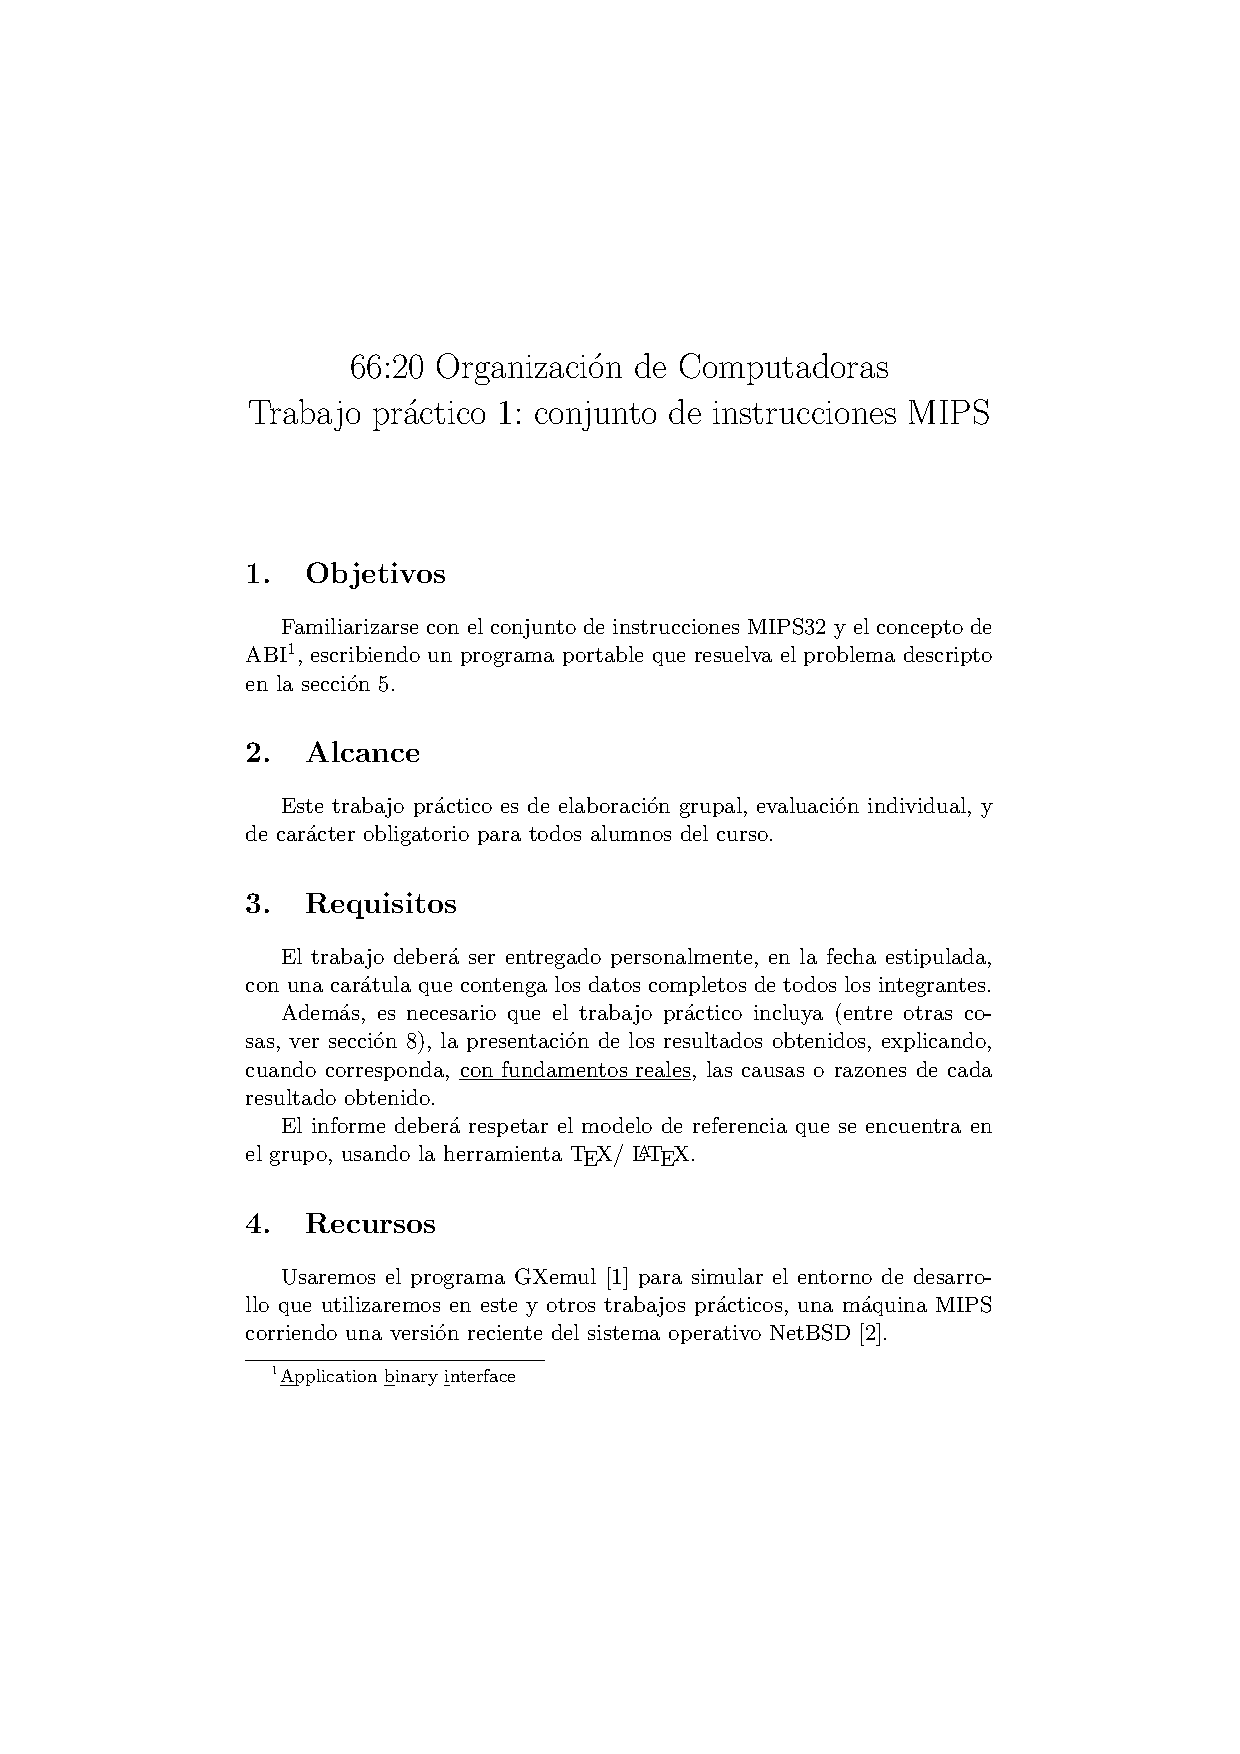
\includepdf[pages=-]{tp1-q2-2017.pdf}

\end{document}
